\documentclass[12pt,a4paper]{article}
\usepackage{amsmath,amssymb,mathrsfs,tikz,times,pifont}
\usepackage{enumitem}
\newcommand\circitem[1]{%
\tikz[baseline=(char.base)]{
\node[circle,draw=gray, fill=red!55,
minimum size=1.2em,inner sep=0] (char) {#1};}}
\newcommand\boxitem[1]{%
\tikz[baseline=(char.base)]{
\node[fill=cyan,
minimum size=1.2em,inner sep=0] (char) {#1};}}
\setlist[enumerate,1]{label=\protect\circitem{\arabic*}}
\setlist[enumerate,2]{label=\protect\boxitem{\alph*}}
%%%::::::by chnini ameur :::::::%%%
\everymath{\displaystyle}
\usepackage[left=1cm,right=1cm,top=1cm,bottom=1.7cm]{geometry}
\usepackage[colorlinks=true, linkcolor=blue, urlcolor=blue, citecolor=blue]{hyperref}
\usepackage{array,multirow}
\usepackage[most]{tcolorbox}
\usepackage{varwidth}
\usepackage{float} %pour utiliser l'option [H] qui force l'image à apparaître exactement à l'endroit où elle est placée dans le code.
\tcbuselibrary{skins,hooks}
\usetikzlibrary{patterns}
%%%::::::by chnini ameur :::::::%%%
\newtcolorbox{exa}[2][]{enhanced,breakable,before skip=2mm,after skip=5mm,
colback=yellow!20!white,colframe=black!20!blue,boxrule=0.5mm,
attach boxed title to top left ={xshift=0.6cm,yshift*=1mm-\tcboxedtitleheight},
fonttitle=\bfseries,
title={#2},#1,
% varwidth boxed title*=-3cm,
boxed title style={frame code={
\path[fill=tcbcolback!30!black]
([yshift=-1mm,xshift=-1mm]frame.north west)
arc[start angle=0,end angle=180,radius=1mm]
([yshift=-1mm,xshift=1mm]frame.north east)
arc[start angle=180,end angle=0,radius=1mm];
\path[left color=tcbcolback!60!black,right color = tcbcolback!60!black,
middle color = tcbcolback!80!black]
([xshift=-2mm]frame.north west) -- ([xshift=2mm]frame.north east)
[rounded corners=1mm]-- ([xshift=1mm,yshift=-1mm]frame.north east)
-- (frame.south east) -- (frame.south west)
-- ([xshift=-1mm,yshift=-1mm]frame.north west)
[sharp corners]-- cycle;
},interior engine=empty,
},interior style={top color=yellow!5}}
%%%%%%%%%%%%%%%%%%%%%%%

\usepackage{fancyhdr}
\usepackage{eso-pic}         % Pour ajouter des éléments en arrière-plan
% Commande pour ajouter du texte en arrière-plan
\usepackage{tkz-tab}
\AddToShipoutPicture{
    \AtTextCenter{%
        \makebox[0pt]{\rotatebox{80}{\textcolor[gray]{0.5}{\fontsize{5cm}{5cm}\selectfont PGB}}}
    }
}
\usepackage{lastpage}
\fancyhf{}
\pagestyle{fancy}
\renewcommand{\footrulewidth}{1pt}
\renewcommand{\headrulewidth}{0pt}
\renewcommand{\footruleskip}{10pt}
\fancyfoot[R]{
\color{blue}\ding{45}\ \textbf{2025}
}
\fancyfoot[L]{
\color{blue}\ding{45}\ \textbf{Prof:M. BA}
}
\cfoot{\bf
\thepage /
\pageref{LastPage}}
% Définition de l'encadré adaptatif avec fond jaune
\newtcolorbox{resultbox}{
    colback=red!30, % Fond rouge clair
    colframe=black, % Bordure noire fine
    sharp corners, % Coins nets
    boxrule=0.5pt, % Contour léger
    boxsep=2pt, % Espacement interne
    left=5pt, right=5pt, top=2pt, bottom=2pt, % Marges internes
}
\begin{document}
\renewcommand{\arraystretch}{1.5}
\renewcommand{\arrayrulewidth}{1.2pt}
\begin{tikzpicture}[overlay,remember picture]
\node[draw=blue,line width=1.2pt,fill=purple,text=blue,inner sep=3mm,rounded corners,pattern=dots]at ([yshift=-2.5cm]current page.north) {\begingroup\setlength{\fboxsep}{0pt}\colorbox{white}{\begin{tabular}{|*1{>{\centering \arraybackslash}p{0.28\textwidth}} |*2{>{\centering \arraybackslash}p{0.2\textwidth}|} *1{>{\centering \arraybackslash}p{0.19\textwidth}|} }
\hline
\multicolumn{3}{|c|}{$\diamond$$\diamond$$\diamond$\ \textbf{Lycée de Dindéfélo}\ $\diamond$$\diamond$$\diamond$ }& \textbf{A.S. : 2024/2025} \\ \hline
\textbf{Matière: Mathématiques}& \textbf{Niveau : 1}\textbf{$^{er}$}S2 &\textbf{Date: 16/06/2025} & \textbf{Durée : 4 heures} \\ \hline
\multicolumn{4}{|c|}{\parbox[c]{10cm}{\begin{center}
\textbf{{\Large\sffamily Correction de la composition Du 2$ ^\text{\bf nd} $ Semestre}}
\end{center}}} \\ \hline
\end{tabular}}\endgroup};
\end{tikzpicture}
\vspace{3cm}

\section*{\underline{Correction Exercice 1 :} 4 pts }

Soient \( A \) et \( B \) deux points du plan tels que \( AB = 8\, \text{cm} \).

\begin{enumerate}
    \item Construisons le barycentre \( G \) des points pondérés \( (A; 1) \) et \( (B; 3) \). \hfill \textbf{0{,}1 pt}

    \( \overrightarrow{AG} =\frac{3}{4}\overrightarrow{AB} \) et \( \overrightarrow{BG} =\frac{1}{4}\overrightarrow{BA} \)

\begin{center}
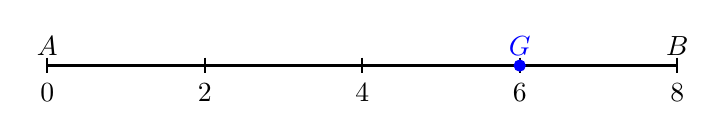
\begin{tikzpicture}
    % Segment de 8 cm
    \coordinate (A) at (0,0);
    \coordinate (B) at (8,0);

    % Tracer le segment AB
    \draw[thick] (A) -- (B);

    % Nommer les extrémités
    \node[above] at (A) {$A$};
    \node[above] at (B) {$B$};

    % Graduations à 2 cm d'intervalle
    \foreach \x in {0,2,4,6,8} {
        \draw[thick] (\x,0.1) -- (\x,-0.1);
        \node[below] at (\x, -0.1) {\x};
    }

    % Placer et nommer le point G à x=6
    \filldraw[blue] (6,0) circle (2pt) node[above] {$G$};
\end{tikzpicture}
\end{center}


    \item Calculons les distances \( GA \) et \( GB \). \hfill \textbf{0{,}5 pt + 0{,}5 pt}

\( 
        \begin{aligned}
                \overrightarrow{AG} =\frac{3}{4}\overrightarrow{AB} &\implies \| \overrightarrow{AG}\| =\frac{3}{4}\|\overrightarrow{AB}\| \\
                                                                    &\implies AG =\frac{3}{4}\times8\\
                                                                    &\implies AG =6\\
        \end{aligned} 
    \)

    \( 
        \begin{aligned}
                \overrightarrow{BG} =\frac{1}{4}\overrightarrow{BA} &\implies \| \overrightarrow{BG}\| =\frac{1}{4}\|\overrightarrow{BA}\| \\
                                                                    &\implies BG =\frac{1}{4}\times8\\
                                                                    &\implies BG =2
        \end{aligned} 
    \)
        \begin{resultbox}
            \[
                \mathbf{GA =6 \text{ et } GB =2}
            \]
		\end{resultbox}
    
    \item Démontrons que pour tout point \( M \) du plan, 
    \[
    MA^2 + 3MB^2 = 4MG^2 + 48
    \]
    \hfill \textbf{0{,}1 pt}

    \(
    \begin{aligned}
    MA^2 + 3MB^2 &= \overrightarrow{MA}^2 + 3\overrightarrow{MB}^2\\
                 &= (\overrightarrow{MG}+\overrightarrow{GA})^2 + 3(\overrightarrow{MG}+\overrightarrow{GB})^2\\
                 &= \overrightarrow{MG}^2+2\overrightarrow{MG}.\overrightarrow{GA}+\overrightarrow{GA}^2+ 3(\overrightarrow{MG}^2+2\overrightarrow{MG}.\overrightarrow{GB}+\overrightarrow{GB}^2)\\
                 &= \overrightarrow{MG}^2+2\overrightarrow{MG}.\overrightarrow{GA}+\overrightarrow{GA}^2+ 3\overrightarrow{MG}^2+6\overrightarrow{MG}.\overrightarrow{GB}+3\overrightarrow{GB}^2\\
                 &= 4\overrightarrow{MG}^2+2\overrightarrow{MG}.\overrightarrow{GA}+6\overrightarrow{MG}.\overrightarrow{GB}+3\overrightarrow{GB}^2+\overrightarrow{GA}^2\\
                 &= 4\overrightarrow{MG}^2+2\overrightarrow{MG}(\overrightarrow{GA}+3\overrightarrow{GB})+3\overrightarrow{GB}^2+\overrightarrow{GA}^2\\
                  &= 4\overrightarrow{MG}^2+2\overrightarrow{MG}(\overrightarrow{O})+3\overrightarrow{GB}^2+\overrightarrow{GA}^2\\
                  &= 4\overrightarrow{MG}^2+3\overrightarrow{GB}^2+\overrightarrow{GA}^2\\
                  &= 4\overrightarrow{MG}^2+3(2)^2+6^2\\
                  &= 4\overrightarrow{MG}^2+12+36\\
                  &= 4MG+48\\
    \end{aligned}
    \)

		        \begin{resultbox}
            \[
                \mathbf{MA^2 + 3MB^2=4MG^2+48\quad\textbf{ CQFD}}
            \]
					\end{resultbox}    
    
    \item Démontrons et construisons l'ensemble des points \( M \) du plan tels que :
    \[
    MA^2 + 3MB^2 = 84
    \]
    \hfill \textbf{0{,}1 pt}

	D'après la relation précédente on a \( MA^2 + 3MB^2=4MG^2+48 \)

		    \(
    \begin{aligned}
    		4MG^2+48 &= 84\\
        4MG^2 &= 84-48\\  
         4MG^2 &=36\\
         MG^2 &=9\\
         MG &=3\\
    \end{aligned}
    \)    
    
    Donc, l'ensemble des points \( M \) tels que \( MA^2 + 3MB^2 = 84 \) est le cercle de centre \( I \) et de rayon \( 3 \) :   
    		    \begin{resultbox}
            \[
                \mathbf{\mathscr{C}(I,\;3) }
            \]
					\end{resultbox} 
    
    \item Déterminons et construison l'ensemble des points \( M \) tels que :
    \[
    \overrightarrow{MA}\cdot\overrightarrow{MB} = -12
    \]
    \hfill \textbf{0{,}1 pt}

		Soit \(I\) milieu de \(AB\)  
		
		\(		
		\begin{aligned}
			\overrightarrow{MA} \cdot \overrightarrow{MB} = -12 &\implies \overrightarrow{MI}^{2}-\frac{\overrightarrow{AB}^{2}}{4} = -12\\
			&\implies \overrightarrow{MI}^{2}-\frac{8^{2}}{4} = -12\\
			&\implies \overrightarrow{MI}^{2}-16 = -12\\
			&\implies \overrightarrow{MI}^{2} = 4\\
		\end{aligned}
		\)  

Donc, l'ensemble des points \( M \) tels que \( \overrightarrow{MA} \cdot \overrightarrow{MB} = -12 \) est le cercle de centre \( I \) et de rayon \( 2 \) :   
    		    \begin{resultbox}
            \[
                \mathbf{\mathscr{C}(I,\;2) }
            \]
					\end{resultbox}  
\end{enumerate}

\section*{\underline{Exercice 2 :} 5 pts}

On considère la fonction \( f \) définie par :
\[
f(x) = \frac{x^2 + ax + b}{x - 1}
\]

\begin{enumerate}
    \item Déterminons les réels \( a \) et \( b \) tels que la courbe \( (C_f) \) passe par le point \( A(0,1) \) et admette en ce point une tangente horizontale. \hfill \textbf{0{,}5 pt + 0{,}75 pt}

    \begin{itemize}
        \item \( (C_f) \) passe par \( A(0,1) \) signifie que \( f(0) = 1 \).\\

        On calcule :
        \[
        f(0) = \frac{0^2 + a \cdot 0 + b}{0 - 1} = \frac{b}{-1} = -b
        \]
        Donc, \( -b = 1 \Rightarrow \boxed{b = -1} \).

        \item \( (C_f) \) admet une tangente horizontale en \( A(0,1) \) signifie que \( f'(0) = 0 \).\\

        On dérive \( f \) par le quotient :
        \[
        f(x) = \frac{u(x)}{v(x)} \quad \text{avec} \quad u(x) = x^2 + ax + b,\quad v(x) = x - 1
        \]
        \[
        f'(x) = \frac{u'(x) \cdot v(x) - u(x) \cdot v'(x)}{(x - 1)^2}
        \]
        \[
        u'(x) = 2x + a, \quad v'(x) = 1
        \]
        \[
        f'(x) = \frac{(2x + a)(x - 1) - (x^2 + ax + b)}{(x - 1)^2}
        \]

        Calculons \( f'(0) \) :

        \[
        f'(0) = \frac{(0 + a)(-1) - (0 + 0 + b)}{1} = \frac{-a - b}{1} = -a - b
        \]

        On veut \( f'(0) = 0 \), donc :
        \[
        -a - b = 0 \Rightarrow -a + 1 = 0 \Rightarrow \boxed{a = 1}
        \]
    \end{itemize}

    Ainsi, les réels recherchés sont \( \boxed{a = 1} \) et \( \boxed{b = -1} \).

    
    On suppose \( a = 1 \) et \( b = -1 \dots \)
    
    \item Déterminons les limites aux bornes de \( \mathcal{D}_f \). Précisons les asymptotes éventuelles. \hfill \textbf{0{,}5 pt + 0{,}5 pt + 0{,}5 pt}

La fonction devient, avec \( a = 1 \) et \( b = -1 \) :
\[
f(x) = \frac{x^2 + x - 1}{x - 1}
\]

\textbf{Domaine de définition} :

    \begin{resultbox}
    \[
    \mathbf{\mathcal{D}_f = \mathbb{R} \setminus \{1\}}
    \]
		\end{resultbox}

\textbf{Limites aux bornes du domaine} :

\begin{itemize}
    \item Limite en \( -\infty \) :

    \[
    \lim_{x \to -\infty} \frac{x^2 + x - 1}{x - 1} = \lim_{x \to -\infty} \frac{x^2(1 + \frac{1}{x} - \frac{1}{x^2})}{x(1 - \frac{1}{x})}
    = \lim_{x \to -\infty} \frac{x(1 + \frac{1}{x} - \frac{1}{x^2})}{1 - \frac{1}{x}} = -\infty
    \]

    Donc :
    \[
    \lim_{x \to -\infty} f(x) = -\infty
    \]

    \item Limite en \( +\infty \) :

    \[
    \lim_{x \to +\infty} \frac{x^2 + x - 1}{x - 1} = +\infty
    \]

    \item Limite en \( 1^- \) :

    \[
    \lim_{x \to 1^-} \frac{x^2 + x - 1}{x - 1} = \frac{1 + 1 - 1}{0^-} = \frac{1}{0^-} = -\infty
    \]

    \item Limite en \( 1^+ \) :

    \[
    \lim_{x \to 1^+} \frac{x^2 + x - 1}{x - 1} = \frac{1 + 1 - 1}{0^+} = \frac{1}{0^+} = +\infty
    \]
\end{itemize}

\textbf{Asymptotes} :
\begin{itemize}
    \item En \( x = 1 \), la fonction tend vers \( \pm\infty \), donc la droite \( x = 1 \) est une \textbf{asymptote verticale}.
\end{itemize}

    
\item Déterminer les réels \( \alpha \), \( \beta \), \( \gamma \) tels que :
\[
f(x) = \alpha x + \beta + \frac{\gamma}{x - 1}
\]
En déduire que la droite \( (D) : y = x + 2 \) est asymptote oblique à la courbe. \hfill \textbf{0{,}75 pt + 0{,}5 pt}

On part de :
\[
f(x) = \frac{x^2 + x - 1}{x - 1}
\]

On effectue la division euclidienne du numérateur par le dénominateur.

\textbf{Division de \( x^2 + x - 1 \) par \( x - 1 \) :}

\[
\frac{x^2 + x - 1}{x - 1} = x + 2 + \frac{1}{x - 1}
\]

Donc :
\[
\boxed{f(x) = x + 2 + \frac{1}{x - 1}} \quad \text{avec } \alpha = 1,\; \beta = 2,\; \gamma = 1
\]

\textbf{Conclusion sur l’asymptote oblique :}

Lorsque \( x \to \pm\infty \), \( \frac{1}{x - 1} \to 0 \), donc : $y = x + 2$

Par conséquent, la droite \( (D) : y = x + 2 \) est une \textbf{asymptote oblique} à la courbe représentative de \( f \).

    
    % À inclure dans le préambule si ce n'est pas encore fait :
% \usepackage{tkz-tab}

\item Dresser le tableau de variations de \( f \) puis tracer la courbe. \hfill \textbf{0{,}1 pt + 0{,}5 pt}

On a vu précédemment que :
\[
f(x) = x + 2 + \frac{1}{x - 1}
\]

On dérive :

\[
f'(x) = \left(x + 2 + \frac{1}{x - 1}\right)' = 1 - \frac{1}{(x - 1)^2}
\]

Étudions le signe de \( f'(x) \) :

\[
f'(x) = \frac{(x - 1)^2 - 1}{(x - 1)^2} = \frac{x^2 - 2x}{(x - 1)^2} = \frac{x(x - 2)}{(x - 1)^2}
\]

\textbf{Tableau de signes de \( f'(x) \) :}

\begin{center}
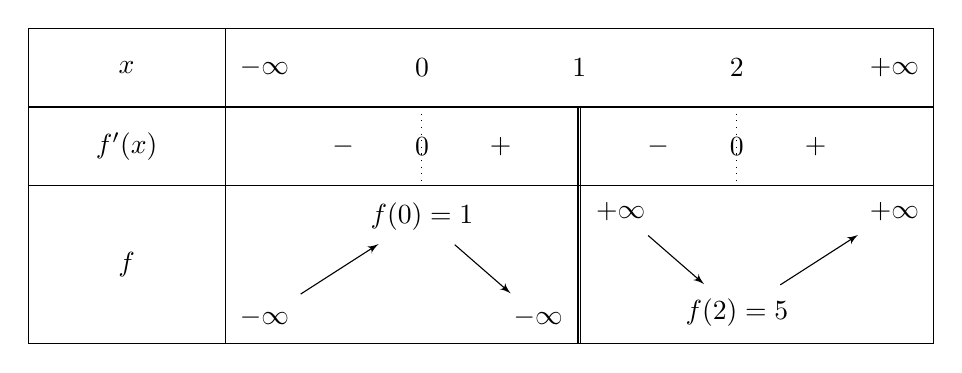
\begin{tikzpicture}
  \tkzTabInit[lgt=2.5,espcl=2]
    {$x$/1, $f'(x)$/1, $f$/2}
    {$-\infty$, $0$, $1$, $2$, $+\infty$}
  \tkzTabLine{ , - , z , + , d , - , z , + }
  \tkzTabVar{-/ $-\infty$ , +/ $f(0) = 1$ , -D+/$-\infty$/$+\infty$ , -/ $f(2) = 5$ , +/ $+\infty$}
\end{tikzpicture}
\end{center}

\textbf{Remarques :}
- En \( x = 1 \), la fonction n'est pas définie (asymptote verticale).

- En \( x = 0 \), \( f(0) = 1 \)

- En \( x = 2 \), \( f(2) = \frac{4 + 2 - 1}{1} = 5 \)

\medskip

\textbf{Courbe représentative :}

Tracer la courbe en tenant compte :

- de l’asymptote verticale \( x = 1 \),

- de l’asymptote oblique \( y = x + 2 \),

- des points remarquables : \( A(0,1) \), \( B(2,5) \).

\begin{center}
\begin{figure}[H]% Forcer l'image à cet endroit
\centering
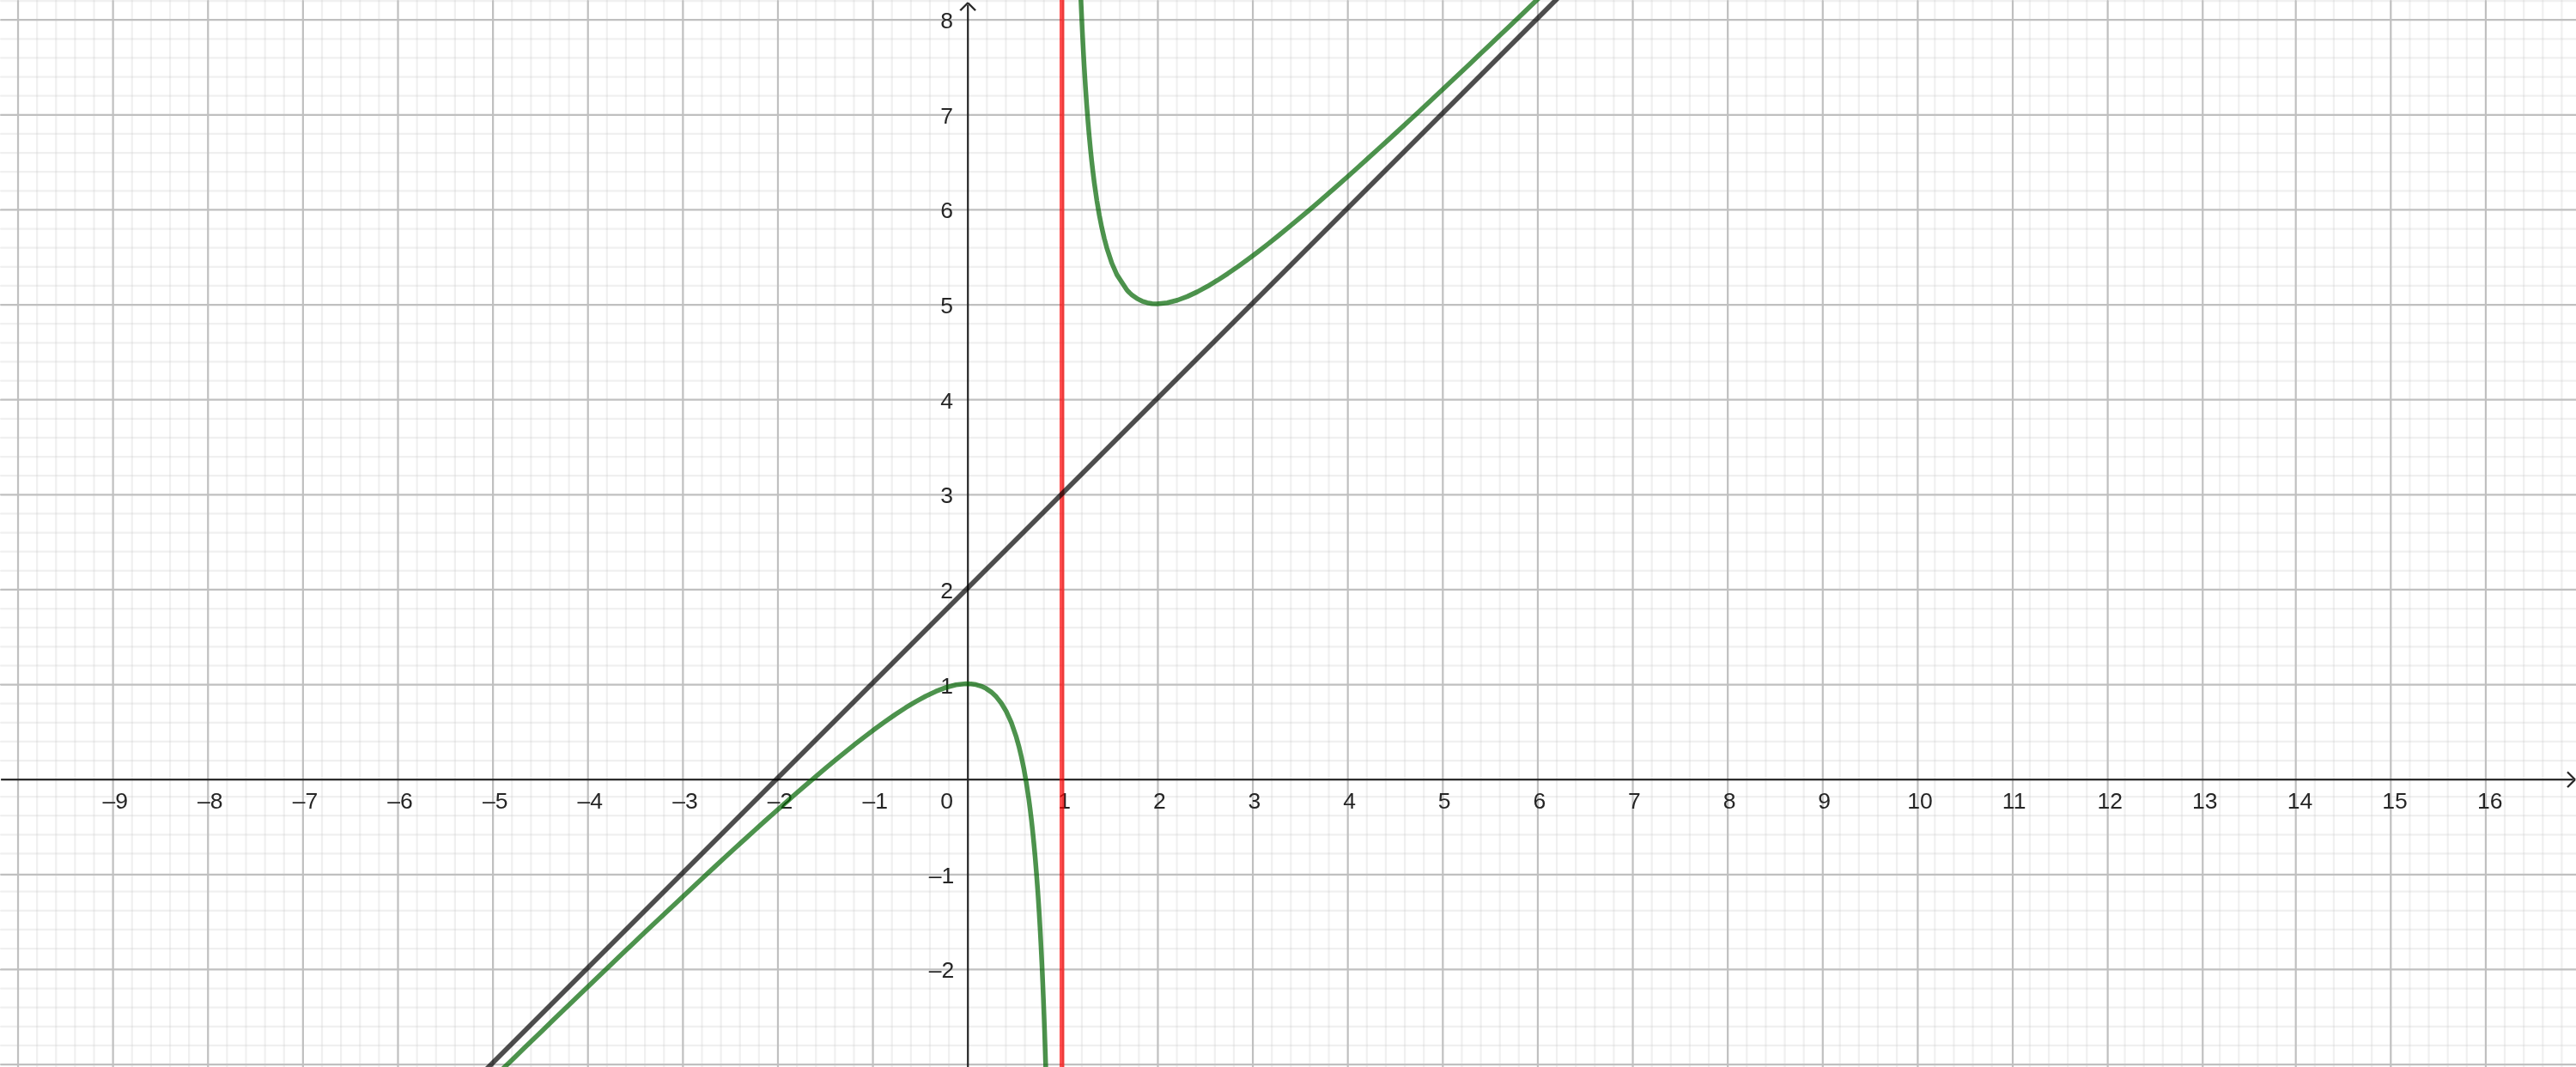
\includegraphics[width=0.8\textwidth]{Compo1erS2.png}
\caption{Représentation graphique de la courbe}
\label{fig:monimage}
\end{figure}
\href{https://www.geogebra.org/classic/rduxvtyf}{Clique ici pour voir la courbe sur géogébra}\\
\end{center}

\end{enumerate}

\section*{Problème : 10 pts}

Soit \( f \) la fonction définie par :
\[
f(x) = 
\begin{cases}
\dfrac{-x^2 + 5x - 5}{x - 1} & \text{si } x \leq 0 \\
\dfrac{3x - 5}{x^2 - 1} & \text{si } x > 0
\end{cases}
\]

\begin{enumerate}
    \item Montrons que \( D_f = \mathbb{R} \setminus \{1\} \). \hfill \textbf{1{,}25 pt}
    \[\textbf{Posons }
f(x) = 
\begin{cases}
f_{1}(x)=\dfrac{-x^2 + 5x - 5}{x - 1} & \text{si } x \leq 0 \\
f_{2}(x)=\dfrac{3x - 5}{x^2 - 1} & \text{si } x > 0
\end{cases}
\]

\( 
\begin{aligned}
f_{1} \exists &\text{ ssi }  x - 1 \neq 0 \text{ et } x \leq 0\\
							&\text{ ssi }  x \neq 1 \text{ et } x \leq 0\\
							&\text{ ssi }  x \neq 1 \text{ et } x \in ]-\infty ; 0]\\
							&\text{ ssi }  1  \notin ]-\infty ; 0]\\
\end{aligned}
\)

Donc \( D_{f_{1}} = ]-\infty ; 0] \)

\( 
\begin{aligned}
f_{2} \exists &\text{ ssi }  x^{2} - 1 \neq 0 \text{ et } x \geq 0\\
							&\text{ ssi }  x \neq -1 \text{ et } x \neq 1 \text{ et } ]0 ;+\infty[\\
							&\text{ ssi }  -1  \notin ]0 ;+\infty[ \text{ et } 1  \in ]0 ;+\infty[\\
							&\text{ ssi }  1  \in ]0 ;+\infty[\\
\end{aligned}
\)

Donc \( D_{f_{2}} = ]0 ; 1[ \cup ]1;+\infty[ \)

\(
\begin{aligned}
D_f &= D_{f_1} \cup D_{f_2} \\
    &= (]-\infty ; 0]) \cup (]0 ; 1[ \cup ]1 ; +\infty[) \\
    &= ]-\infty ; 0] \cup ]0 ; 1[ \cup ]1 ; +\infty[ \\
    &= ]-\infty ; 1[ \cup ]1 ; +\infty[ \\
    &=\mathbb{R}\setminus\{1\}
\end{aligned}
\)

    \begin{resultbox}
    \[
    \mathbf{\mathcal{D}_f = \mathbb{R} \setminus \{1\}}
    \]
		\end{resultbox}

\textcolor{red}{\textbf{Autre Méthode}}		

    \textbf{Étude du domaine de définition de \( f_1 \) :}

    L'expression \( f_1(x) = \dfrac{-x^2 + 5x - 5}{x - 1} \) est définie si \( x - 1 \neq 0 \), soit \( x \neq 1 \).\\
    Or, \( f_1 \) est définie uniquement sur \( x \leq 0 \), donc comme \( 1 \notin ]-\infty ; 0] \), on a :
    \[
    D_{f_1} = ]-\infty ; 0]
    \]

    \textbf{Étude du domaine de définition de \( f_2 \) :}

    L'expression \( f_2(x) = \dfrac{3x - 5}{x^2 - 1} \) est définie si \( x^2 - 1 \neq 0 \), soit \( x \neq \pm 1 \).\\
    Comme \( f_2 \) est définie pour \( x > 0 \), il faut exclure \( x = 1 \), mais \( x = -1 \) ne fait pas partie de l'intervalle.\\
    Donc :
    \[
    D_{f_2} = ]0 ; 1[ \cup ]1 ; +\infty[
    \]

    \textbf{Conclusion :}
    \[
    D_f = D_{f_1} \cup D_{f_2} = ]-\infty ; 0] \cup \left( ]0 ; 1[ \cup ]1 ; +\infty[ \right) = \mathbb{R} \setminus \{1\}
    \]

    \[
    \boxed{D_f = \mathbb{R} \setminus \{1\}}
    \]
		
		
    \item Calculons les limites aux bornes de \( D_f \). \hfill \textbf{0{,}1 pt}

		\textbf{\underline{En $-\infty$}:} 

		\(
		\begin{aligned}
				\lim_{x\to -\infty}f_{1}(x)&=\lim_{x\to -\infty}\frac{-x^{2}+5x-5}{x-1}\\
																	 &=\lim_{x\to -\infty}\frac{-x^{2}}{x}\\
																	 &=\lim_{x\to -\infty}-x\\
																	 &=+\infty
		\end{aligned}
		\)		

    \begin{resultbox}
    \[
    \mathbf{\lim_{x\to -\infty}f(x) = +\infty}
    \]
		\end{resultbox}		
		
		\textbf{\underline{En $+\infty$}:} 

		\(
		\begin{aligned}
				\lim_{x\to +\infty} f_{2}(x)&=\lim_{x\to +\infty}\frac{3x-5}{x^{2}-1}\\
																		&=\lim_{x\to +\infty}\frac{3x}{x^{2}}\\
																		&=\lim_{x\to +\infty}\frac{3}{x}\\
																		&=0
		\end{aligned}
		\)		

    \begin{resultbox}
    \[
    \mathbf{\lim_{x\to +\infty}f(x) = 0}
    \]
		\end{resultbox}	

		\begin{center}
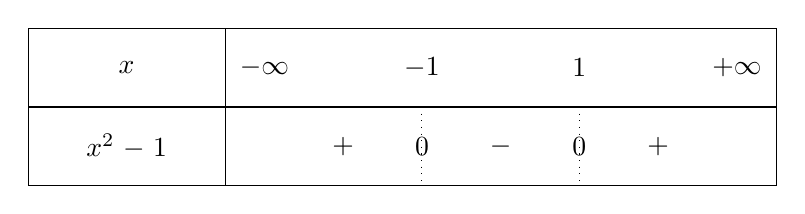
\begin{tikzpicture}
  \tkzTabInit[lgt=2.5,espcl=2]
    {$x$/1, $x^{2}-1$/1}
    {$-\infty$, $-1$, $1$, $+\infty$}
  \tkzTabLine{ , + , z , - , z , + }
\end{tikzpicture}
\end{center}		
		
		\textbf{\underline{En $1^{-}$}:}

		\(
		\begin{aligned}
				\lim_{x\to 1^{-}} f_{2}(x)&=\lim_{x\to 1^{-}}\dfrac{3x-5}{x^{2}-1}\\
																	&=\lim_{x\to 1^{-}}\dfrac{-2}{0^{-}}\\
																	&=+\infty
		\end{aligned}
		\)		

    \begin{resultbox}
    \[
    \mathbf{\lim_{x\to 1^{-}}f(x) = +\infty}
    \]
		\end{resultbox}		
		
		\textbf{\underline{En $1^{+}$}:}   

		\(
		\begin{aligned}
					\lim_{x\to 1^{+}} f_{2}(x)&=\lim_{x\to 1^{+}}\dfrac{3x-5}{x^{2}-1}\\
																		&=\lim_{x\to 1^{+}}\dfrac{-2}{0^{+}}\\
																		&=-\infty
		\end{aligned}
		\)    
    
    \begin{resultbox}
    \[
    \mathbf{\lim_{x\to 1^{+}}f(x) = -\infty}
    \]
		\end{resultbox}    
    
    \item Déduisons-en les asymptotes de \( (C_f) \). \hfill \textbf{0{,}5 pt}
    
    \begin{itemize}
    \item La limite en \( +\infty \) est nulle, donc la droite \( y = 0 \) est une \textbf{asymptote horizontale} à droite.
    \item La fonction tend vers \( \pm\infty \) en \( x = 1 \), donc la droite \( x = 1 \) est une \textbf{asymptote verticale}.
		\end{itemize}
		 \begin{resultbox}
    	\[
    	\mathbf{y = 0 \text{ est une AH en } +\infty, \quad x = 1 \text{ est une AV}}
    	\]
		\end{resultbox} 
    
    \item Montrons que la droite d’équation \( y = -x + 4 \) est asymptote oblique à \( (C_f) \) en \( -\infty \). \hfill \textbf{0{,}5 pt}
    
    On considère : \( f_1(x) = \frac{-x^2 + 5x - 5}{x - 1} \)

		Une division euclidienne donne : \( \frac{-x^2 + 5x - 5}{x - 1} = -x + 4 + \frac{-1}{x - 1} \)

		Donc : \( f_1(x) = -x + 4 + \frac{-1}{x - 1} \)


Or, \(\lim_{x \to -\infty} \frac{-1}{x - 1} = 0\), donc : \( \lim_{x \to -\infty} f_1(x) = -x + 4 \)

Ainsi, la droite \( y = -x + 4 \) est une \textbf{asymptote oblique} à gauche.

		 \begin{resultbox}
    	\[
    	\mathbf{y = -x + 4 \text{ est une asymptote oblique en } -\infty}
    	\]
		\end{resultbox} 

\textcolor{red}{ \textbf{Autre Méthode} }

D'après la question \textbf{2)} \( \lim\limits_{x\to -\infty} f(x) = +\infty \) donc cherchons \( \lim\limits_{x\to -\infty} \frac{f(x)}{x} \)

\(
\begin{aligned}
	\lim_{x \to -\infty} \frac{f(x)}{x} &= \lim_{x \to -\infty} \frac{\frac{-x^2 + 5x - 5}{x - 1}}{x}\\
														&= \lim_{x \to -\infty} \frac{-x^2 + 5x - 5}{x^{2} - x}\\
														&= \lim_{x \to -\infty} \frac{-x^2}{x^{2}}\\
														&= -1\\
\end{aligned}
\)    

Comme \( \lim_{x \to -\infty} \frac{f(x)}{x} = -1 \) donc cherchons \( \lim_{x \to -\infty} [ f(x) - (-x) ] \)

En effet :

\(
\begin{aligned}
	\lim_{x \to -\infty} [ f(x) + (-x) ] &= \lim_{x \to -\infty} \frac{-x^2 + 5x - 5}{x - 1}+x\\
														&= \lim_{x \to -\infty} \frac{-x^2 + 5x - 5+x^{2}-x}{x - 1}\\
														&= \lim_{x \to -\infty} \frac{5x - 5-x}{x - 1}\\
														&= \lim_{x \to -\infty} \frac{4x - 5}{x - 1}\\
														&=4
\end{aligned}
\) 

\begin{resultbox}
\[
\lim_{x \to -\infty} [f(x) + x] = 4
\quad \Rightarrow \quad \boxed{y = -x + 4 \text{ est une asymptote oblique à gauche}}
\]
\end{resultbox}    
    
    \item Étudier la continuité de \( f \) en \( 0 \). \hfill \textbf{0{,}75 pt}

\(
\begin{aligned}
f(0) &= \frac{-0 + 0 - 5}{0 - 1}\\
		 &= \frac{-5}{-1}\\
		 &= 5
\end{aligned}
\)

\(
\begin{aligned}
\lim_{x \to 0^-} f(x) &= \lim_{x \to 0^-} \frac{-x^2 + 5x - 5}{x - 1}\\
											&= \frac{0 + 0 - 5}{0 - 1}\\
											&= 5
\end{aligned}
\)

\(
\begin{aligned}
\lim_{x \to 0^+} f(x) &= \lim_{x \to 0^+} \dfrac{3x - 5}{x^2 - 1}\\
											&= \dfrac{0 - 5}{0 - 1}\\ 
											&= \dfrac{-5}{-1}\\ 
											&= 5 
\end{aligned}
\)

\begin{resultbox}
\[
\boxed{\text{Donc } \lim_{x \to 0^-} f(x) = \lim_{x \to 0^+} f(x) = f(0) = 5 \implies f \text{ est continue en } x = 0}
\]
\end{resultbox}

    
    \item Étudions la dérivabilité de \( f \) en \( 0 \) puis interpréter graphiquement les résultats. \hfill \textbf{0{,}1 pt + 0{,}5 pt}

On calcule les limites du taux d'accroissement à gauche et à droite de 0 :

\textbf{\underline{En $0^{-}$}:}  \( f(x) = \dfrac{-x^2 + 5x - 5}{x - 1} \)

\(
\begin{aligned}
\lim_{x \to 0^-}\dfrac{f(x) - f(0)}{x - 0} &= \lim_{x \to 0^-}\dfrac{f(x) - 5}{x}\\
																					  &= \lim_{x \to 0^-}\dfrac{\frac{-x^2 + 5x - 5}{x - 1} - 5}{x} \\
																						&= \lim_{x \to 0^-}\dfrac{\frac{-x^2 + 5x - 5 - 5(x - 1)}{x - 1}}{x} \\
																						&= \lim_{x \to 0^-}\dfrac{\frac{-x^2 + 5x - 5 - 5x + 5}{x - 1}}{x} \\
																						&= \lim_{x \to 0^-}\dfrac{\frac{-x^2}{x - 1}}{x}\\ 
																						&= \lim_{x \to 0^-}\dfrac{-x^2}{x(x - 1)} \\
																						&= \lim_{x \to 0^-}\dfrac{-x^2}{x(x - 1)} \\
																						&= \lim_{x \to 0^-}\dfrac{-x}{x - 1} \\
																						&= 0
\end{aligned}
\)

\textbf{\underline{En $0^{+}$}:}  \( f(x) = \dfrac{3x - 5}{x^2 - 1} \)

\(
\begin{aligned}
\lim_{x \to 0^+}\dfrac{f(x) - f(0)}{x} &= \lim_{x \to 0^+}\dfrac{\frac{3x - 5}{x^2 - 1} - 5}{x} \\
																			 &= \lim_{x \to 0^+}\lim_{x \to 0^+}\dfrac{\frac{3x - 5 - 5(x^2 - 1)}{x^2 - 1}}{x} \\
																			 &= \lim_{x \to 0^+}\dfrac{\frac{3x - 5 - 5x^2 + 5}{x^2 - 1}}{x}\\ 
																			 &= \lim_{x \to 0^+}\frac{\frac{3x - 5x^2}{x^2 - 1}}{x} \\
                                       &= \lim_{x \to 0^+}\frac{3x - 5x^2}{x(x^2 - 1)} \\
																			 &= \lim_{x \to 0^+} \frac{3x - 5x^2}{x(x^2 - 1)}\\ 
																			 &= \lim_{x \to 0^+} \frac{3 - 5x}{x^2 - 1}\\
																			 &= -3
\end{aligned}
\)

\textbf{Conclusion} :

\[
\lim_{x \to 0^-} \frac{f(x) - f(0)}{x} = 0 \neq -3 = \lim_{x \to 0^+} \frac{f(x) - f(0)}{x}
\]

\begin{resultbox}
\[
\boxed{f_{g}'(0)\neq f_{d}'(0) \text{ donc }  f \text{ n’est pas dérivable en } x = 0}
\]
\end{resultbox}

\textbf{Interprétation graphique :}

\( f \) est continue en \( x = 0 \) mais non dérivable en en \( x = 0 \)

\begin{itemize}
 \item \( \lim_{x \to 0^-}\dfrac{f(x) - f(0)}{x - 0} = 0 \) donc \( (C_f) \) admet une démi-tangeante horizontale en \( 0\) d'équation \( y = 0 \)
 \item \( \lim_{x \to 0^+}\dfrac{f(x) - f(0)}{x - 0} = -3 \) donc \( (C_f) \) admet une démi-tangeante horizontale en \( 0 \) d'équation \( y = -3x \)
\end{itemize} 
    
    
    \item Calculons \( f'(x) \) pour \( x < 0 \) et pour \( x > 0 \). \hfill \textbf{0{,}5 pt + 0{,}5 pt}

\textbf{Pour \( x < 0 \), on a :} \( f(x) = f_1(x) = \frac{-x^2 + 5x - 5}{x - 1} \)

\[
\begin{aligned}
f_1'(x) &= \frac{(-2x + 5)(x - 1) - (-x^2 + 5x - 5)(1)}{(x - 1)^2}
\end{aligned}
\]

\[
\begin{aligned}
f_1'(x) &= \frac{(-2x + 5)(x - 1) + x^2 - 5x + 5}{(x - 1)^2} \\
&= \frac{(-2x^2 + 2x + 5x - 5) + x^2 - 5x + 5}{(x - 1)^2} \\
&= \frac{-2x^2 + 7x - 5 + x^2 - 5x + 5}{(x - 1)^2} \\
&= \frac{-x^2 + 2x}{(x - 1)^2}
\end{aligned}
\]

\[
\boxed{f'(x) = \dfrac{-x^2 + 2x}{(x - 1)^2} \quad \text{pour } x < 0}
\]

\bigskip

\textbf{Pour \( x > 0 \), on a :} \( f(x) = f_2(x) = \frac{3x - 5}{x^2 - 1} \)

\[
\begin{aligned}
f_2'(x) &= \frac{3(x^2 - 1) - (3x - 5)(2x)}{(x^2 - 1)^2}
\end{aligned}
\]

\[
\begin{aligned}
f_2'(x) &= \frac{3x^2 - 3 - (6x^2 - 10x)}{(x^2 - 1)^2} \\
&= \frac{3x^2 - 3 - 6x^2 + 10x}{(x^2 - 1)^2} \\
&= \frac{-3x^2 + 10x - 3}{(x^2 - 1)^2}
\end{aligned}
\]

\[
\boxed{f'(x) = \dfrac{-3x^2 + 10x - 3}{(x^2 - 1)^2} \quad \text{pour } x > 0}
\]

\begin{resultbox}
\[
f'(x) = 
\begin{cases}
f_{1}'(x)=\dfrac{-x^2 + 2x}{(x - 1)^2} & \text{si } x \leq 0 \\
f_{2}'(x) = \dfrac{-3x^2 + 10x - 3}{(x^2 - 1)^2} & \text{si } x > 0
\end{cases}
\]
\end{resultbox}

    \item Étudions le signe de \( f'(x) \) pour \( x < 0 \) puis pour \( x > 0 \). \hfill \textbf{0{,}5 pt + 0{,}5 pt}

\textbf{Pour \( x < 0 \), on a :}
\[
f'(x) = \frac{-x^2 + 2x}{(x - 1)^2}
\]

Le dénominateur \( (x - 1)^2 > 0 \) pour tout \( x \neq 1 \), donc le signe de \( f'(x) \) est celui du numérateur :
\[
\begin{aligned}
-x^2 + 2x &= -x(x - 2)
\end{aligned}
\]

\textbf{Étude du signe de \( -x(x - 2) \) sur \( ]-\infty ; 0[ \)} :

\begin{center}
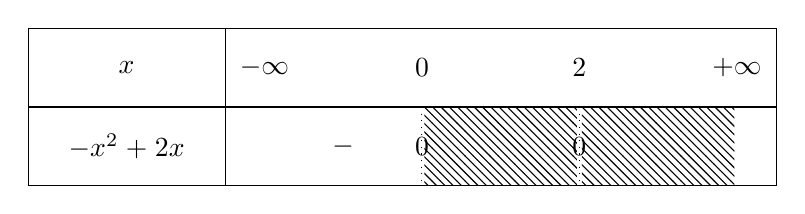
\begin{tikzpicture}
  \tkzTabInit[lgt=2.5,espcl=2]
    {$x$/1, $-x^2 + 2x$/1}
    {$-\infty$, $0$, $2$, $+\infty$}
  \tkzTabLine{ , - , z , h , z , h }
\end{tikzpicture}
\end{center}	

\[
\boxed{f'(x) < 0 \quad \text{pour tout } x \in ]-\infty ; 0[}
\]

\bigskip

\textbf{Pour \( x > 0 \), on a :}
\[
f'(x) = \frac{-3x^2 + 10x - 3}{(x^2 - 1)^2}
\]

Le dénominateur est strictement positif pour \( x \in \mathbb{R} \setminus \{-1, 1\} \), et ici \( x > 0 \), donc le signe de \( f'(x) \) est celui du numérateur :
\(
 -3x^2 + 10x - 3
\)

\textbf{Étudions le signe } :

\[
\begin{aligned}
\Delta &= 10^2 - 4 \times (-3) \times (-3) = 100 - 36 = 64 \\
x_1 &= \frac{-10 - \sqrt{64}}{2 \times (-3)} = \frac{-10 - 8}{-6} = \frac{-18}{-6} = 3 \\
x_2 &= \frac{-10 + \sqrt{64}}{2 \times (-3)} = \frac{-10 + 8}{-6} = \frac{-2}{-6} = \dfrac{1}{3}
\end{aligned}
\]


\begin{center}
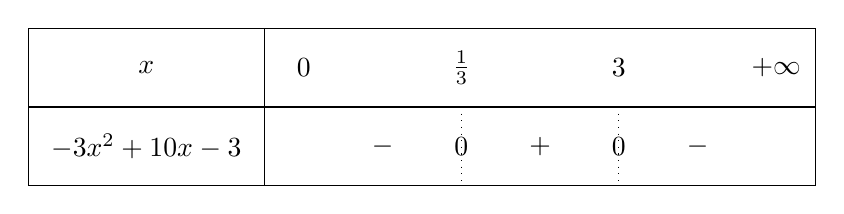
\begin{tikzpicture}
  \tkzTabInit[lgt=3,espcl=2]
    {$x$/1, $-3x^2 + 10x - 3$/1}
    {$0$, $\frac{1}{3}$, $3$, $+\infty$}
  \tkzTabLine{ , - , z , + , z , - }
\end{tikzpicture}
\end{center}

\[
\boxed{
f'(x) < 0 \text{ sur } ]0 ; \tfrac{1}{3}[ \cup ]3 ; +\infty[,
\quad f'(x) > 0 \text{ sur } ]\tfrac{1}{3} ; 3[
}
\]


    \item Dressons le tableau de variation de \( f \). \hfill \textbf{1{,}5 pt}

\begin{center}
\begin{tikzpicture}
  \tkzTabInit[lgt=2.5,espcl=2]
    {$x$/1, $f'(x)$/1, $f$/2}
    {$-\infty$, $0$, $\frac{1}{3}$, $1$, $3$, $+\infty$}
  \tkzTabLine{ ,  - , d , - , z , + , d ,+, z, - }
  %\tkzTabVar{+/ $+\infty$ , -/ $5$, -/$f(\dfrac{1}{3})$ , +D-/$+\infty$/$-\infty$ , +/ $f(3)$ , -/ $0$}
  %\tkzTabVar{+/ $+\infty$ , -/ $5$, -/ $\dfrac{9}{2}$ , +D-/$+\infty$/$-\infty$ , +/ $\dfrac{1}{2}$ , -/ $0$}
  \tkzTabVar{+/ $+\infty$ , / , -/ $\dfrac{9}{2}$ , +D-/$+\infty$/$-\infty$ , +/ $\dfrac{1}{2}$ , -/ $0$}
\end{tikzpicture}
\end{center}

    %\item Construire \( (C_f) \). \hfill \textbf{0{,}1 pt}
\end{enumerate}
\end{document}